
\subsection{\sinterface}
The \astaff[] interface is illustrated in figure \ref{fig:staff_interface}.
After login, the \astaff[] is presented with the \textit{main} window. 

\begin{figure}[p]
	\centering
		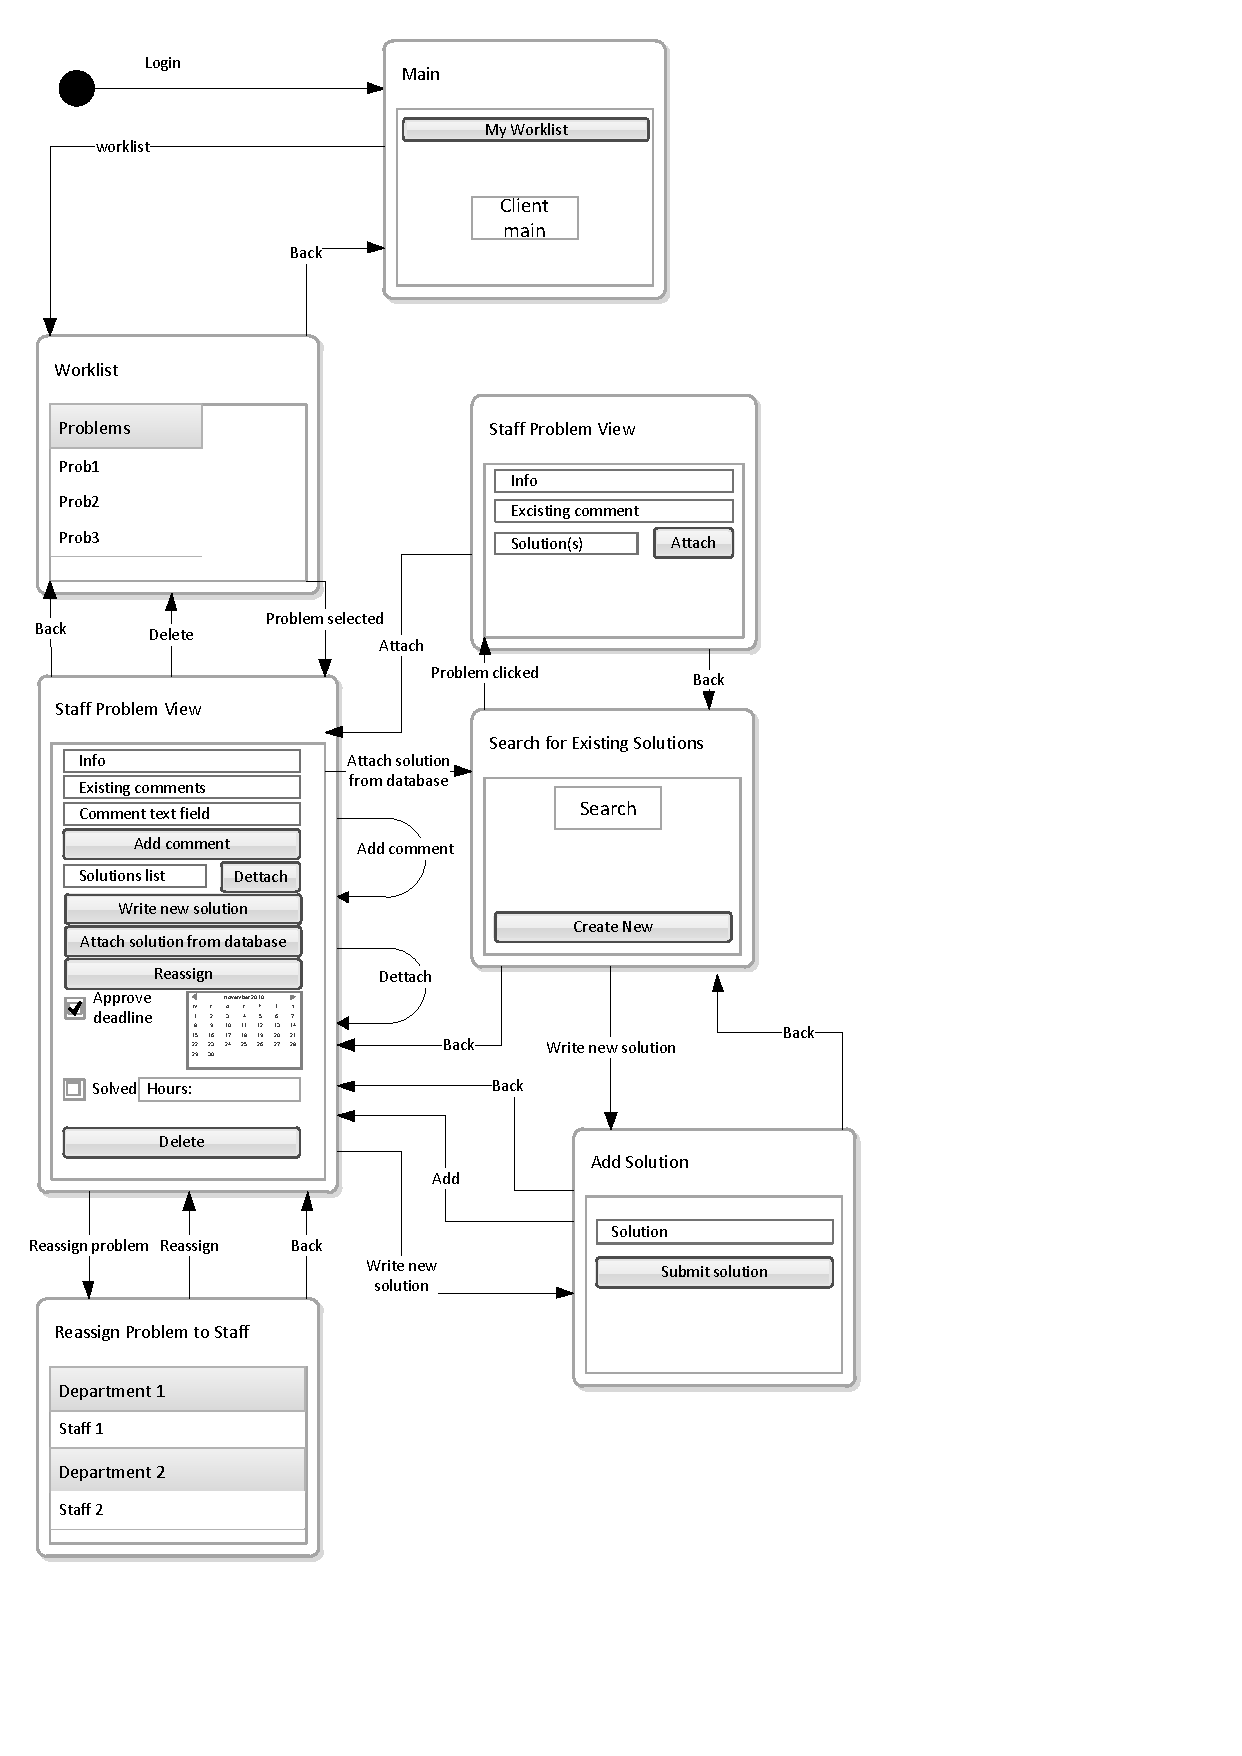
\includegraphics[width = \textwidth, clip=true, trim=0 4cm 5cm 0]{input/application_domain_analysis/Navigation_DiagramStaff.pdf}
	\morscaption{The navigation diagram of the staff interface}
	\label{fig:staff_interface} %fig:Navigation_DiagramAdmin
\end{figure}

\subsubsection{Main}
The staff main window give the \astaff[] member access to all the functionality from the \astaff[] interface and from the \aclient[] interface. The \astaff[] have one button:
\begin{itemize}
	\item ``My Worklist'' which directs the \astaff[] member to the ``Worklist'' window. 
\end{itemize}   
Plus the menu buttons from the \aclient[]s main menu.

%After login the staff is presented with the ``Main'' staff window where the button ``Worklist'' is shown. When the ``Worklist'' button is press the window ``Worklist'' opens. 


\subsubsection{Worklist}
The ``Worklist'' is a list of all the problem assigned to a specific \astaff[] member. The window has the following elements:
\begin{itemize}
	\item A list with all the problems assigned to the \astaff[] member who is signed in.
\end{itemize}
The list show the following properties: Name, Deadline, Priority, and ETC.
When a problem is clicked the window ``Staff problem view'' opens. 


\subsubsection{Staff Problem View}
This window shows all the information related to a specific problem. 
The ``Staff problem view'' features the following:
\begin{itemize}
	\item The window contains a text field which contains information about the problem
	\item A text field with all the existing comments related to the problem.
	\item A text field where new comments can be entered.
	\item The button ``Create comment'' to send the entered comment.
	\item A text field containing none or more solutions.
	\item The button ``Attach solution from database'' which send the \astaff[] to ``Search for existing solutions''.  
	\item The ``Reassign'' button which opens the ``Reassign problem to staff'' window.
	\item A checkbox to mark the problem as solved.
	\item A calendar to set deadlines.
	\item The checkbox ``Approve deadline'' approves a suggested deadline if one is suggested.
	\item The button ``Write new solution'' which sends the \astaff[] to ``Add solution''
\end{itemize}

\subsubsection{Search for Existing Solutions}
This window enables the staff to search for existing solutions among existing problems. The ``Search for existing solutions'' window contains the following elements:
\begin{itemize}
	\item The ``Search'' window from the \aclient[] interface \ref{sec:client_interface} is reused, and it enables the \astaff[] to search for problems.
	\item The button ``Create New'' which sends the \astaff[] to the ``Add solution'' window.
\end{itemize} 
If a problem is double click the \astaff[] is send to ``Staff problem view''.

\subsubsection{Staff Problem View}
The ``Staff Problem View'' show properties of the selected problem. This window contains the following:
\begin{itemize}
	\item A text field with relevant information about the problem.
	\item A text field with all the existing comments related to the problem.
	\item A text field containing none or more solutions.
	\item The button ``Attach'' inserts the selected solution into the solutions list from ``Staff Problem View'', and the \astaff[] is send to the ``Staff Problem View'' window.
\end{itemize}

\subsubsection{Add Solution}
The ``Add Solution'' window allows the \staff[] to enter a new solution. The window contains the following elements:
\begin{itemize}
	\item A text field where the new solution can be entered.
	\item The ``Add'' button which sends the entered solution to the Solution list in the ``Staff Problem View'' window, the \astaff[] is send to the ``staff Problem View'' window.
\end{itemize}
 


